\title{Identifying Breast Cancer Gene Signatures with Feature Selection}
\author{
        \textsc{Gustavo Empinotti}
            \qquad
        \textsc{Susan Tu}
            \qquad
        \textsc{Raf Mertens}
        \mbox{}\\ %
        \\
        CS229\\
        \mbox{}\\ %
        \normalsize
            \texttt{gustavoe}
        \textbar{}
            \texttt{susanctu}
        \textbar{}
            \texttt{rafm}
        \normalsize
            \texttt{@stanford.edu}
}
\date{\today}
\documentclass[11pt]{article}
%\documentclass{acmconf}
\usepackage[pdftex]{graphicx}
\usepackage[paper=a4paper,dvips,top=2.5cm,left=1.5cm,right=1.5cm,
    foot=1cm,bottom=2.5cm]{geometry}
%----------------------------------------------------------
\begin{document}

\maketitle

\begin{abstract}
Statistical or machine learning methods have been used to find cancer gene signatures intended to predict survival or to classify patient prognosis as good/poor. However, a recent paper suggests that random gene subsets perform as well or better than 47 published gene signatures obtained through statistical methods, perhaps because cancer disrupts expression of many genes not directly related to cancer \cite{venet}. In this paper, we use different feature selection methods in an attempt to find a small set of genes that distinguishes normal breast tissue from malignant tumor tissue. We plan to compare the predictive power of our selected genes to that of random gene subsets, gene subsets that should be unrelated to cancer, and previously published gene signatures.

%In this paper, we use different feature selection methods to identify the most important genes that distinguish normal breast tissue from malignant tumor tissue. We plan to compare the predictive power of our selected genes to that of random gene subsets, gene subsets that should be unrelated to cancer, and previously published gene signatures. Our methods include forward feature selection, backward feature selection, and sparse regression. We find that ... works best and we are able to distinguish cancer tissue from normal tissue with an accuracy of ... \%. 


\end{abstract}

\section{Introduction}

Microarray technology has allowed for significant improvements in determining which genes’ expression correlate with specific diseases. In particular, much work has been done in using gene expression data to predict cancer survival [1,2] or classify types or subtypes of cancer [1,3,4]. Popular approaches include machine learning techniques (such as entropy theory), 2 and t-statistics for feature selection followed by k-nearest-neighbors, and Naive Bayes and SVM for classification [5]. While some authors have verified that their results are better than random, however, Venet \emph{et al.} report that some authors who assume a null hypothesis of no association between a randomly selected gene signature and survival have published gene signatures that do not perform significantly better (or even perform worse) than a randomly selected signature [6].%FIXME:hard-coded references

In this paper, we describe our attempts to use feature selection to identify a gene signature for breast cancer. The data set, provided to us by Professor David Dill, was originally obtained from the National Cancer Institute’s Cancer Genome Atlas and includes expression data of 17814 genes from 599 people, of whom 533 have breast cancer and 66 do not. Data was obtained from Agilent G4502 microarrays. 

\section{Methods}
\setcounter{subsection}{-1} %this makes it so that preprocessing is 2.0 so that 2.1 and 3.1 both refer to forward selection
\subsection{Preprocessing} 
Expression data was normalized to have mean 0 and standard deviation 1. At least one gene expression value was missing for each of 319 people; These values collectively pertrained to 537 distinct genes and there were a total of 1740 missing values in total.We set these values to be equal to the mean, 0. \\

TODO for final report: describe methods
\subsection{Forward Selection}
The most straightforward method for feature selection is forward selection: rank the features by some score, then select a specified number of the highest-ranking features, or select all features that have a score higher than some cutoff. We ranked the genes by Chi2 statistic and selected the 50 highest ranking features. The Chi2 statistic measures the dependence between random variables, so we select the features that are least likely to be independent of class. One downside of this method is that if 2 relevant features are (nearly) identical, we select both even though really only one of the two gives us new information.
%\subsection{Backwards Selection}

%\subsection{Logistic Regression}

\section{Results \& Discussion}

\subsection{Forward Selection}
We clearly observe the phenomenon of selecting multiple very similar features described above. For example selecting the 50 most relevant features using all our data results in the following list of genes:\\\\
'HLA-DRB5' 'HLA-DRB6' 'HLA-E' 'HLA-F' 'HLA-G' 'HLCS' 'HMG2L1' 'HMGCS2'
 'HMHB1' 'HMOX2' 'HMP19' 'HMX2' 'HN1' 'HN1L' 'HNMT' 'HNRNPC' 'HNRNPU'
 'HNRPCL1' 'HOXA6' 'HOXA7' 'HOXA9' 'HOXB1' 'HOXB2' 'HOXB3' 'HOXB6' 'HOXC10'
 'HOXC11' 'HOXC12' 'HOXC13' 'HOXC4' 'LOC92345' 'SLC7A13' 'SLC9A10'
 'SLC9A3R1' 'SLC9A3R2' 'SLC9A4' 'SLC9A7' 'SLC9A8' 'SLC9A9' 'SLCO1C1'
 'SLFN12' 'SLFN13' 'SLFN5' 'SLFNL1' 'SLIC1' 'SLIT2' 'SLIT3' 'SLITRK3'
 'SLITRK4' 'SLK'
 
Many of which are obviously related (e.g. HOXC11, HOXC12, ...).\\\\
To measure the prediction power of our model we used 4-fold cross validation. To do this, we only use the training data to do feature selection, since we otherwise encode information about the test data into our model. Using a SVM we get the following results averaged over the 4 fold cross validation parts (the results for an SVM trained using all features and again tested using 4-fold cross validation are included for comparison):\\

\begin{tabular}{r | c l c }
    & Chi2 Top 50 & All Features\\
  \hline 
    Accuracy & 0.984998675 & 0.911570558 \\
    Precision & 0.985778285 & 0.909611142 \\
    Recall & 0.998120301 & 1.0 \\
  
\end{tabular}
\subsection{Backwards Selection}
\subsection{Logistic Regression}

\begin{figure}[h!]
  \centering
    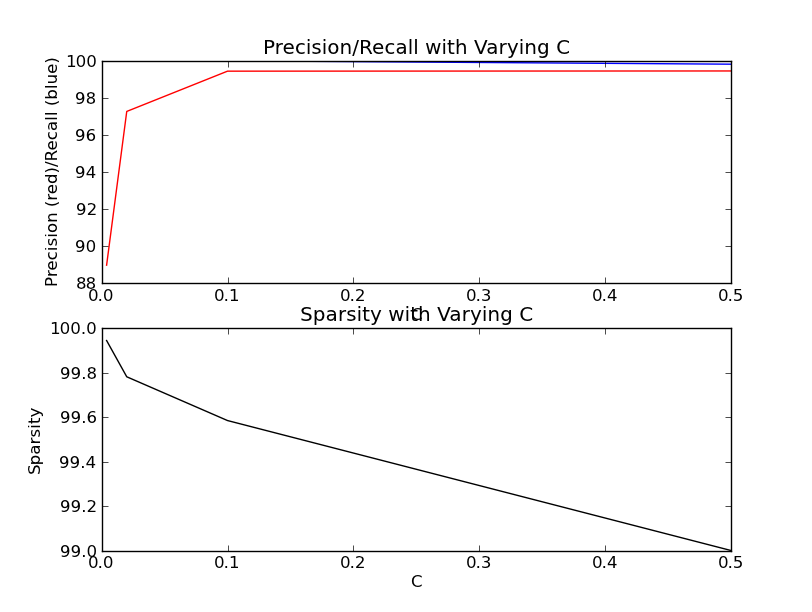
\includegraphics[scale=0.3]{sparselog.png}
  \caption{Results of logistic regression with l1 regularization. Precision, recall, and sparsity shown are averages resulting from 4-fold cross-validation.}
\label{fig:sparselog}
\end{figure}

%will not be including huge lists of genes in the final doc, but since we haven't evaluated these lists yet, just putting them here as what-we-have-so-far
The precision and recall for a logistic regression with no regularization were 0.995 and 0.996. As can be seen in Figure \ref{fig:sparselog}, C=0.01 provides reasonable precision/recall while still providing a reasonably small number of selected features. The genes selected when C=0.01 when training on a random 3-quarters of our dataset were $[$'ACVR1C', 'ADAMDEC1', 'ADH4', 'AKR1C1', 'AMIGO2', 'ANKRD22', 'ANLN', 'AREG', 'ASPA', 'ASPN', 'BUB1', 'C6orf156', 'CA4', 'CEACAM6', 'CEP55', 'CES1', 'CITED1', 'COL10A1', 'COL11A1', 'CST1', 'CXCL11', 'CXCL2', 'CXCL3', 'DAZ4', 'FABP1', 'FAM111B', 'FAM3B', 'FLJ35773', 'FLJ45557', 'GGTA1', 'GJB2', 'GSTA2', 'HEMGN', 'HLA-DPB1', 'HMGCLL1', 'IGSF10', 'INHBA', 'JAKMIP1', 'KIF14', 'LRRC3B', 'MMP1', 'MMP11', 'MMP13', 'MMP3', 'MUCL1', 'NPNT', 'NPY2R', 'OCA2', 'PDK4', 'PPAPDC1A', 'PTPRR', 'S100B', 'S100P', 'SDPR', 'SEMA3A', 'SFRP1', 'SNCA', 'SULT2A1', 'SYT13', 'TDO2', 'TFPI2', 'TNMD', 'TSLP', 'USP44', 'VCX3A', 'WISP1'$]$.

Taking the intersection of all the gene lists generated during cross-validation, we found that the genes that appear in all four of these lists are $[$'COL10A1', 'AREG', 'WISP1', 'COL11A1', 'TNMD', 'GJB2', 'PPAPDC1A', 'CA4', 'SYT13', 'SFRP1', 'TFPI2', 'FAM111B', 'MMP3', 'MMP11'$]$. However, it is worrying that there is so little overlap with the gene lists obtained from forward selection.

\subsection{Random Subsets}

However, we find that we can achieve near-perfect precision/recall with random subsets as well. The following numbers are from training a SVM in 4-fold cross-validation with random subsets of 50 genes:
\begin{tabular}{ l | c }
    Precision & Recall\\
  \hline 
    1.0 & 1.0 \\
    0.993 & 0.971 \\
    0.992 & 0.985 \\
    0.985 & 1.0 \\
  \hline
\end{tabular}
\section{Conclusion}
From these preliminary results, we conclude that while distinguishing between normal and cancerous tissue is easy to do, finding a gene signature in which the genes are actually related to cancer pathology is difficult because In fact, we saw that a random subset of 50 genes can provide good predictive power. We plan to consult the literature and Professor Dill for advice on how to proceed. 

\section{Acknowledgements}
Thank you to Professor David Dill (Stanford, Department of Computer Science) for data and guidance and to and Professor Stephen Boyd (Stanford, Department of Electrical Engineering) for his guidance.

\begin{thebibliography}{9}
\bibitem{haibe} Haibe-Kains, B., Desmedt, C., Piette, F., Buyse, M., Cardoso, F., van't Veer, L., \& Sotiriou, C. (2008). Comparison of prognostic gene expression signatures for breast cancer. BMC Genomics, 91-9. doi:10.1186/1471-2164-9-394

\bibitem{buyse} Buyse, M., Loi, S., van't Veer, L., Viale, G., Delorenzi, M., Glas, A. M., \& ... Piccart, M. J. (2006). Validation and Clinical Utility of a 70-Gene Prognostic Signature for Women With Node-Negative Breast Cancer. JNCI: Journal Of The National Cancer Institute, 98(17), 1183-1192. doi:10.1093/jnci/djj329

\bibitem{sotiriou} Sotiriou, C., \& Pusztai, L. (2009). Gene-Expression Signatures in Breast Cancer. New England Journal Of Medicine, 360(8), 790-800. doi:10.1056/NEJMra0801289

\bibitem{Abraham} Abraham, G., Kowalczyk, A., Loi, S., Haviv, I., \& Zobel, J. (2010). Prediction of breast cancer prognosis using geneset statistics provides signature stability and biological context. BMC Bioinformatics,11277-291. doi:10.1186/1471-2105-11-277

\bibitem{liu} Liu, H., Li, J., \& Wong, L. (2002). A comparative study on feature selection and classification methods using gene expression profiles and proteomic patterns. Genome Informatics. International Conference On Genome Informatics, 1351-60.

\bibitem{venet} Venet, D., Dumont, J. E., \& Detours, V. (2011). Most Random Gene Expression Signatures Are Significantly Associated with Breast Cancer Outcome. Plos Computational Biology, 7(10), 1-8. doi:10.1371/journal.pcbi.1002240

\end{thebibliography}
\end{document}
